\documentclass[10pt, a4paper, twocolumn]{article} % 10pt font size (11 and 12 also possible), A4 paper (letterpaper for US letter) and two column layout (remove for one column)

%%%%%%%%%%%%%%%%%%%%%%%%%%%%%%%%%%%%%%%%%
% Wenneker Article
% Structure Specification File
% Version 1.0 (28/2/17)
%
% This file originates from:
% http://www.LaTeXTemplates.com
%
% Authors:
% Frits Wenneker
% Vel (vel@LaTeXTemplates.com)
%
% License:
% CC BY-NC-SA 3.0 (http://creativecommons.org/licenses/by-nc-sa/3.0/)
%
%%%%%%%%%%%%%%%%%%%%%%%%%%%%%%%%%%%%%%%%%

%----------------------------------------------------------------------------------------
%	PACKAGES AND OTHER DOCUMENT CONFIGURATIONS
%----------------------------------------------------------------------------------------

\usepackage[english]{babel} % English language hyphenation

\usepackage{microtype} % Better typography

\usepackage{amsmath,amsfonts,amsthm} % Math packages for equations

\usepackage[svgnames]{xcolor} % Enabling colors by their 'svgnames'

\usepackage[hang, small, labelfont=bf, up, textfont=it]{caption} % Custom captions under/above tables and figures

\usepackage{booktabs} % Horizontal rules in tables

\usepackage{lastpage} % Used to determine the number of pages in the document (for "Page X of Total")

\usepackage{graphicx} % Required for adding images

\usepackage{url} % url loading

\usepackage{enumitem} % Required for customising lists
\setlist{noitemsep} % Remove spacing between bullet/numbered list elements

\usepackage{sectsty} % Enables custom section titles
\allsectionsfont{\usefont{OT1}{phv}{b}{n}} % Change the font of all section commands (Helvetica)

%----------------------------------------------------------------------------------------
%	MARGINS AND SPACING
%----------------------------------------------------------------------------------------

\usepackage{geometry} % Required for adjusting page dimensions

\geometry{
	top=1cm, % Top margin
	bottom=1.5cm, % Bottom margin
	left=2cm, % Left margin
	right=2cm, % Right margin
	includehead, % Include space for a header
	includefoot, % Include space for a footer
	%showframe, % Uncomment to show how the type block is set on the page
}

\setlength{\columnsep}{7mm} % Column separation width

%----------------------------------------------------------------------------------------
%	FONTS
%----------------------------------------------------------------------------------------

\usepackage[T1]{fontenc} % Output font encoding for international characters
\usepackage[utf8]{inputenc} % Required for inputting international characters

\usepackage{XCharter} % Use the XCharter font

%----------------------------------------------------------------------------------------
%	HEADERS AND FOOTERS
%----------------------------------------------------------------------------------------

\usepackage{fancyhdr} % Needed to define custom headers/footers
\pagestyle{fancy} % Enables the custom headers/footers

\renewcommand{\headrulewidth}{0.0pt} % No header rule
\renewcommand{\footrulewidth}{0.4pt} % Thin footer rule

\renewcommand{\sectionmark}[1]{\markboth{#1}{}} % Removes the section number from the header when \leftmark is used

%\nouppercase\leftmark % Add this to one of the lines below if you want a section title in the header/footer

% Headers
\lhead{} % Left header
\chead{\textit{\thetitle}} % Center header - currently printing the article title
\rhead{} % Right header

% Footers
\lfoot{} % Left footer
\cfoot{} % Center footer
\rfoot{\footnotesize Page \thepage\ of \pageref{LastPage}} % Right footer, "Page 1 of 2"

\fancypagestyle{firstpage}{ % Page style for the first page with the title
	\fancyhf{}
	\renewcommand{\footrulewidth}{0pt} % Suppress footer rule
}

%----------------------------------------------------------------------------------------
%	TITLE SECTION
%----------------------------------------------------------------------------------------

\newcommand{\authorstyle}[1]{{\large\usefont{OT1}{phv}{b}{n}\color{DarkRed}#1}} % Authors style (Helvetica)

\newcommand{\institution}[1]{{\footnotesize\usefont{OT1}{phv}{m}{sl}\color{Black}#1}} % Institutions style (Helvetica)

\usepackage{titling} % Allows custom title configuration

\newcommand{\HorRule}{\color{DarkGoldenrod}\rule{\linewidth}{1pt}} % Defines the gold horizontal rule around the title

\pretitle{
	\vspace{-30pt} % Move the entire title section up
	\HorRule\vspace{10pt} % Horizontal rule before the title
	\fontsize{32}{36}\usefont{OT1}{phv}{b}{n}\selectfont % Helvetica
	\color{DarkRed} % Text colour for the title and author(s)
}

\posttitle{\par\vskip 15pt} % Whitespace under the title

\preauthor{} % Anything that will appear before \author is printed

\postauthor{ % Anything that will appear after \author is printed
	\vspace{10pt} % Space before the rule
	\par\HorRule % Horizontal rule after the title
	\vspace{20pt} % Space after the title section
}

%----------------------------------------------------------------------------------------
%	ABSTRACT
%----------------------------------------------------------------------------------------

\usepackage{lettrine} % Package to accentuate the first letter of the text (lettrine)
\usepackage{fix-cm}	% Fixes the height of the lettrine

\newcommand{\initial}[1]{ % Defines the command and style for the lettrine
	\lettrine[lines=3,findent=4pt,nindent=0pt]{% Lettrine takes up 3 lines, the text to the right of it is indented 4pt and further indenting of lines 2+ is stopped
		\color{DarkGoldenrod}% Lettrine colour
		{#1}% The letter
	}{}%
}

\usepackage{xstring} % Required for string manipulation

\newcommand{\lettrineabstract}[1]{
	\StrLeft{#1}{1}[\firstletter] % Capture the first letter of the abstract for the lettrine
	\initial{\firstletter}\textbf{\StrGobbleLeft{#1}{1}} % Print the abstract with the first letter as a lettrine and the rest in bold
}

%----------------------------------------------------------------------------------------
%	BIBLIOGRAPHY
%----------------------------------------------------------------------------------------

%\usepackage[backend=bibtex,style=authoryear,natbib=true]{biblatex} % Use the bibtex backend with the authoryear citation style (which resembles APA)
\usepackage[backend=bibtex,style=nature,natbib=true,maxbibnames=99]{biblatex}

\addbibresource{terminusdb.bib} % The filename of the bibliography

\usepackage[autostyle=true]{csquotes} % Required to generate language-dependent quotes in the bibliography

\usepackage{etoolbox}
\apptocmd{\sloppy}{\hbadness 10000\relax}{}{}

 % Specifies the document structure and loads requires packages

\newcommand{\s}[1]{\textcolor{Blue}{#1}}
\newcommand{\p}[1]{\textcolor{Red}{#1}}
\newcommand{\w}[1]{\textcolor{Green}{#1}}

\title{Succinct Data Structures and Delta Encoding for Modern Databases}

\author{
  \authorstyle{Matthijs van Otterdijk\textsuperscript{1,2} and Gavin Mendel-Gleason\textsuperscript{1,3} and Kevin Feeney\textsuperscript{1,4}}
  \newline\newline
  \textsuperscript{1}\institution{DataChemist Ltd. {\protect\url{http://datachemist.com}}}\\
  \textsuperscript{2}\institution{\protect\url{matthijs@datachemist.com}}\\
  \textsuperscript{3}\institution{\protect\url{gavin@datachemist.com}}\\
  \textsuperscript{4}\institution{\protect\url{kevin@datachemist.com}}
}

\date{\today}

\begin{document}

\maketitle

\thispagestyle{firstpage}

\lettrineabstract{Modern hardware architectures includes larger main
  memory and pervasive parallelism. Modern software development
  processes now incorporate continuous integration/continuous
  delivery (CI/CD) coupled with version control. These fundamental
  changes to information technology infrastructure necessitate a
  re-appraisal of database architecture.  TerminusDB makes a radical
  departure from historical architectures to address these
  changes. First, we implement a graph database with a strong schema
  so as to retain both simplicity and generality of design. Second, we
  implement this graph using succinct immutable data structures which
  enable more sparing use of main memory resources. Prudent use of
  memory reduces cache contention while read-only data structures
  simplify parallel access significantly.  Third, we adopted the
  delta encoding approach to updates as is used in source control systems
  such as git. This provides transaction processing and updates to our
  immutable database data structures, recovering standard database
  management features while also providing in addition the whole suite
  of revision control features: branch, merge, squash, rollback, blame
  and time-travel facilitating CI/CD approaches on data.}

\section{Introduction}

There has been an explosion of new database designs, including graph
databases, key-value stores, document databases and multi-model
databases. Yet the majority of production databases are still based on
the RDBMS designs of the 1970s\cite{Codd:1970:RMD:362384.362685}.

Meanwhile both hardware infrastructure and software design process
have moved on significantly over the course of the last 40 years. In
particular machines with terrabytes of RAM are now available for
prices reasonable enough for some small and medium sized enterprises.

At the same time flexible revision control systems have revolutionised
the software development process. The maintenance of histories, of
records of modification and the ability to roll back enables engineers
to have confidence in making modificiations collaboratively. This is
augmented with important features such as branching, labelling,
rebasing, and cloning. When combined with continuous integration/continuous
delivery\cite{65147}\cite{LAUKKANEN201755} (CI/CD) teams of
programmers can have confidence that central repositories are
maintained in correct states once testing and verification of have
been passed.

These two developments suggest a solution at their
intersection. Namely the use of in-memory immutable {\em succinct}
data structures and {\em deltas} as used in revision control
systems. TerminusDB demonstrates how these features can be combined to
produce a flexible transactional graph database. 

\section{Design}

TerminusDB is a full featured graph database management system (GDBMS)
including a rich query language: WOQL (the Web Object Query Language).
However, we restrict our attention here to the underlying
datastructure design and layout which we have implemented in a
Rust\cite{Blandy:2015:RPL:3019371} library which we call {\em{terminus-store}}.

We describe in turn the graph database model which is used, the
succinct data structure approach, and finally how we implement
revision control type operations using {\em deltas} which we collect
together with some metadata into an object which we term {\em layers}.

\subsection{Graph Databases}

Graph databases are one of the fastest growing of the new database
paradigms\cite{}. Since graphs are very general it is possible to
render many database modeling techniques in a graph database. The
simplicity and generality make it a good candidate for a {\em general
purpose} change set orientated approach to an online transaction
processing database.

The TerminusDB infrastucture is based on the {\em RDF} standard. This
standard specifies finite labelled directed graphs which are
parameteric in some universe of datatypes. The names for nodes and
labels are drawn from a set of IRIs (Internationalized Resource
Identifiers). For TerminusDB we have chosen the {\em XSD} datatypes as
our universe of concrete values.

More formally, in TerminusDB a graph \(G\) is a set of triples drawn
from the set \( IRI \times IRI \times (IRI \oplus XSD)\) where \(IRI\)
is a set of valid IRIs and \(XSD\) is the set of valid XSD values.
While some RDF databases allow multiplicity of triples (i.e. a bag),
the choice of a set simplifies transaction processing in our setting.

For schema design TerminusDB uses the OWL language, with two
modifications to make it suitable as a schema language. Namely we
dispense with the open world interpretation and insist on the unique
name assumption\cite{DBLP:journals/semweb/FeeneyMB18}. This provides
us with a rich modelling language which can provide constraints on the
allowable shapes in the graph.

TerminusDB, following on from the RDF tradition, is not a property
graph. However it can model properties using an intermediate nodes and
this pattern can be made explicit in the OWL schema design. Again this
choice leads to simplicity of the underlying representation, which, as
we will see is important when constructing succinct data structures
with change sets.

\subsection{Succinct Data Structures}

Succinct data structures\cite{Jacobson:1988:SSD:915547} are a family of
data structures which are close in size to the information theoretic
minimum representation. Technically they can be defined as data structures
whose size is:

\[ n + o(n) \]

Where \(n\) is the information theoretic minimum size. Succinct
representations are generally somewhat more computationally expensive
than less compact representations with pointers when working with
small problems. However, as the size of the datastructure grows, the
ability to avoid new cache reads at various levels of the memory
hierarchy (including reading information from disk) means that these
representations can prove very speed
competitive\cite{doi:10.1002/spe.2198} in practice.

TerminusBD largely borrows its graph data structure design from
HDT\cite{10.1007/978-3-642-30284-8_36} with some modifications which
simplify the use of change sets. The authors originally evaluated HDT
as a possibility for a graph which was too large to fit in memory when
loaded into postgresql and found that queries on the resulting graph
performed very well in practice.

In particular, the primary datastructures of the HDT format are
retained, namely {\em front coded dictionaries}, {\em bit sequences}
and {\em wavelet trees}.

\subsubsection{Plain Front-Coding Dictionary}

Due to the unusual quantity of shared prefixes found in RDF data due
to the nature of URIs and IRIs, front-coding provides a fast
dictionary format with significant compression of
data\cite{MARTINEZPRIETO201673}.

The primary operations exposed by the datastructure are {\em
  string-id} which gives us a natural number corresponding with the
string, and {\em id-string} which gives a string corresponding with a
natural number.

\begin{table}
	\centering
	\begin{tabular}{l|rl}
		\toprule
		String & Offset & Remainder \\
		\midrule
        Pearl Jam & 0 & Pearl Jam \\
        Pink Floyd & 1 & ink Floyd \\
        Pixies & 2 & xies \\
		The Beatles & 0 & The Beatles \\
		The Who & 4 & Who \\
		\bottomrule
	\end{tabular}
    \caption{Plain Front Coding Dictionary}
    \label{tab:pfc}
\end{table}

The data strucure sorts the strings and allows sharing of prefixes by
reference to the number of characters from the preceeding strings
which are shared. An example is given in Table~\ref{tab:pfc}. The
position in the dictionary gives us the implicit natural number
identifier.

\subsubsection{Succinct Graphs Encoding}

Once subject, object and property of an edge have been appropriately
converted into integers by use of the subject-object dictionary, the
value dictionary and the predicate dictionary, we can use these
integers to encode the triples using bit sequences.

Succinct sequences encode sequences drawing from some alphabet
\(\sigma\). In the case of a bit-sequence, \(\sigma=\{0,1\}\). They
typically expose (at least) the following primitives:

\begin{itemize}
\item \(rank(a, S, i)\) which counts occurances of \(a\) in the sequence from \(S[0,i]\).
\item \(select(a, S, i)\) which returns the location of the \(i\)-th
  occurance of \(a\) in the sequence \(S\).
\item \(access(S, i)\) which returns the symbol at \(S[i]\).
\end{itemize}

Given a sorted set of triples, for each subject identifier, in order
from \(\{0..n\}\) where \(n\) is the number of triples, we emit a
\(1\) followed by a \(0\) for every predicate associated in a triple
with that subject. We then produce a vector of all predicates used and
the association with the subject is apparent from the position of
zeros in the bit sequence.

We repeat the process for predicates and objects resulting in a
complete encoded for our triples. We can see an example in
Table~\ref{tab:graph}.  We have written the vectors in this table so
that the triples are vertically aligned, with subjects in blue,
predicates in red and objects in green in order to make the encoding
easier to see. The subject ids are actually implicit in the number of
\(1\)s encoding in the subject bit sequence and are only written in
the table for clarity.

\begin{table}
	\centering
	\begin{tabular}{l|l|l}
		\toprule
		Triples & Encoding & \\
		\midrule
        \(  (\s{1},\p{2},\w{3}) \)  & \(\s{1}\;\;\;\;\s{2} \;\;\;\;\s{3}\) & Subject Ids \\
        \(  (\s{1},\p{2},\w{4}) \)  & \(   1\;\;\;\;    1\;    0\;    1\) & Encoded Subject Bit Sequence\\
        \(  (\s{2},\p{3},\w{5}) \)  & \(\p{2}\;\;\;\;\p{3}\;\p{4}\;\p{5}\) & Predicate Vector \\
	    \(  (\s{2},\p{4},\w{6}) \)  & \(   1\;   0\;    1\;    1\;    1\) & Encoded Predicate Bit Sequence\\
	    \(  (\s{3},\p{5},\w{7}) \)  & \(\w{3}\;\w{4}\;\w{5}\;\w{6}\;\w{7}\) & Object Vector \\
		\bottomrule
	\end{tabular}
    \caption{Succinct Graph Representation}
    \label{tab:graph}
\end{table}

This format allows fast lookup of triples based on query modes in
which the subject identifier is known, as we can use \(select\) to
find the position in the predicate vector and subsequently use the
predicate identifier to \(select\) in the object vector. We use a
wavelet tree to enable search starting from the predicate. Details of
this can be found in \cite{10.1007/978-3-642-30284-8_36}.

\subsection{Delta Encoded Databases}

The use of {\em delta encoding} in software development is now
ubiquitous due to the enormous popularity of the {\em git} revision
control system which makes use of these techniques to store histories
of revisions.

Git stores objects which contain either the complete dataset of
interest or the information about what is updated (deleted / added) as
a delta. All changes to the source control system are thereby simply
management problems of these objects.

This approach exposes a number of very powerful operations to sofware
developers collaborating on a code base. The operations include:

\begin{itemize}
\item {\bf History} Since new updates are actually layered over previous
  ones, developers can {\em time travel}, looking into the past,
  rolling back to the past, or even reapplying changes to current
  versions.
\item {\bf Branching} Developers can create a derived version of a given
  code-base where additional operations can be performed without
  disrupting the original.
\item {\bf Merging} When two branches diverge, the changes can be merged
  into a single version by choosing a strategy for combining changes.
\end{itemize}

TerminusDB uses an analogous approach to updates. A given database is
comprised of {\em layers} which stands in place of the objecs of
git. Each layer has a unique identifier, a 20-byte name. The base
layer contains a simple graph represented using the succinct data
strucures already described earlier.

\begin{figure}
	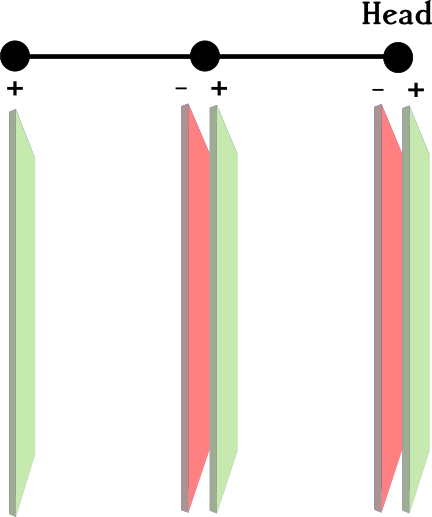
\includegraphics[width=\linewidth]{layers-diagram.png} % Figure image
	\caption{A graph composed of layers} % Figure caption
	\label{fig:layers} % Label for referencing with \ref{bear}
\end{figure}

Above this layer, we can have further layers. Each additional layer
above the base layer is comprised of additional dictionaries for newly
added subjects and objects, predicates or values.

It also contains the index structures used for the base graph to
represent {\em positive} edges which have been added to the graph. And
we have a membership set of {\em negative} edges which describe those
triples which have been deleted as shown in Figure~\ref{fig:layers}.

Each layer has a pointer to the previous layer which is achieved by
referring to its 20-byte name.

This immutable chain strucure allows for straightforward uncoordinated
multi-read access.  It also allows for easy branching. Any number of
new layers, for instance can point to the same former parent layer
without impact.

In order to manage these layers as datastores, we use a {\em label}. A
label is a name which points to one of the 20-byte identifiers. In the
present implementation this is a file with the name of the label
containing the 20-byte identifier.

\subsubsection{Dictionary modfications}

Due to the use of delta encodings, new triples can be added which are
not present in the original dictionary. We therefore start new
dictionaries with a recorded offset, remembering the last bucket from
the previous dictionary.

\subsection{Write Transactions}

When an update transaction is initiated, a new {\em layer builder} is
created, which logs all newly inserted or deleted edges. When this
{\em layer builder} is committed, it yields a {\em layer} which has
organised the insertions in our succinct data structures.

In TerminusDB we require that graphs conform to the constraints
imposed by the OWL description of the dataset. This means that we
produce a hypothetical database by committing the layer builder
without advancing head. First we check the constraints hold on this
new intermediate database and after these are passed, it is safe to
advance head to this newly created layer. {\em Advancing} is done by
side-effecting the label to point to the new 20-byte value. The
problem of coordination in the face of side-effects is reduced to the
problem of label management, simplifying much of the architecture. A
schematic of the workflow of the write transaction is given in
Figure~\ref{workflow}.

\begin{figure}
	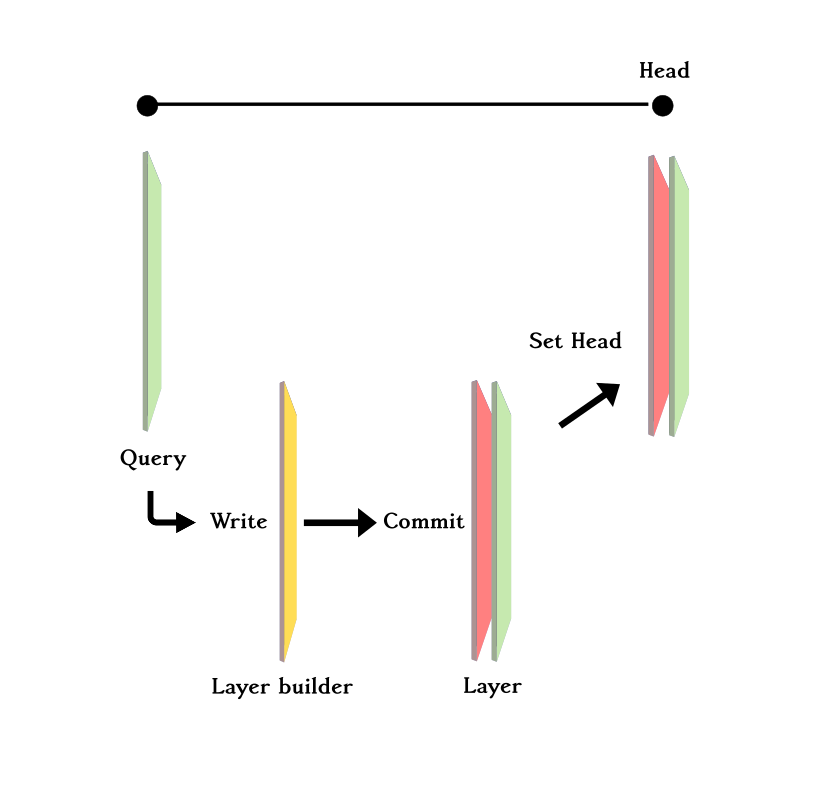
\includegraphics[width=\linewidth]{query_write_commit_head} % Figure image
	\caption{Write transaction workflow} % Figure caption
	\label{workflow} % Label for referencing with \ref{bear}
\end{figure}

% More here. 

\subsection{Delta compression}

As new updates are performed the database layer depth increases. Since
the layers are essentially arranged as linked lists. This will incur a
performance penalty requiring repeated searching for every query. In
order to improve performance, it is possible to perform a {\em delta
  compression} as is used in git, or even to recalculate the full
dataset as a new base-layer. In git this step can be performed
manually, or it will occur with a default depth threshold is passed.

Since the layers are immutable, this operation can be done
concurrently. Commis that occur before the process is completed simply
layer over the squash commit with no visible change in the content of
the database.

Compressed deltas of this type can allow older layers to be archived,
or even deleted. The removal of previous layers removes the capacity
to time-travel or to track whether the database arose from a
branch. However, this information can be kept seperately in a metadata
repository, as is the plan for future version of TerminusDB.

\section{Future Work}

Values are stored as strings using a plain front coding dictionary
uniformly for all data types. Obviously this is less than ideal in
that it causes an expansion in size for the storage of integers, dates
and other specific types. It also means that only search from the
beginning of the string is fast. In future versions of store we hope
to differentiate our indexing strategies for the various datatypes in
XSD.

For strings the use of succinct data structure immediately suggests a
potential candidate: the
FM-index\cite{Ferragina:2005:ICT:1082036.1082039}. With FM-indexing
very large datasets could still have reasonable query times for
queries which are typically done on full text indexes using inverted
term-document indexing. We have yet to explore the candidates for
numeric and date types.

Currently the tracking of history and branches is implicit. We intend
to adopt a more explicit approach, storing a graph of the various
commits coupled with timestamps and other metadata which will
facilitate effective management.

\section{Conclusion}

The use of advanced CI/CD workflows for databases as yet has not been
practical due to the lack of tool-chain support. In the software world
we have seen just what a large impact appropriate tools can make with
advent of git.

TerminusDB makes possible these collaborative CI/CD type operations in
the universe of data management.

This is made possible because of the synergies which an immutable
layered approach has with the {\em succinct datastructure} approach
that we have used for encoding.

TerminusDB provides a practical tool for enabling branch, merge,
rollback and the various automated and manual testing regimes which
are faciliated by them on a transactional database management system
which can provide sophisticated query support.

\printbibliography[title={Bibliography}]

\end{document}
